\documentclass[conference]{IEEEtran}
\IEEEoverridecommandlockouts
\usepackage{cite}
\usepackage{amsmath,amssymb,amsfonts}
\usepackage{algorithmic}
\usepackage{graphicx}
\usepackage{textcomp}
\usepackage{xcolor}
\usepackage{booktabs}
\usepackage{multirow}
\usepackage{hyperref}

\def\BibTeX{{\rm B\kern-.05em{\sc i\kern-.025em b}\kern-.08em
    T\kern-.1667em\lower.7ex\hbox{E}\kern-.125emX}}

\begin{document}

\title{Adaptive Token-Aware KV Cache Compression with Asymmetric Key/Value Quantization Granularity}

\author{
\IEEEauthorblockN{Chandan Munjal}
\IEEEauthorblockA{\textit{Independent Research} \\
chandanmunjal@gmail.com}
}

\maketitle

\begin{abstract}
The key/value (KV) cache is the dominant memory cost of autoregressive transformer
inference at long context lengths, and hard-eviction compression methods (e.g.\ H2O)
permanently discard tokens that may later become relevant again. We present
\textit{AdaptiveKVCache}, a drop-in HuggingFace \texttt{transformers} cache that never
evicts a token but instead continuously reassigns each cached token to one of three
precision tiers -- FP16, INT8, or INT4 -- based on a running, exponentially-decayed
importance score, so that a token demoted to low precision can be promoted back to FP16
if it becomes important again. Within the quantized tiers we further apply
\emph{asymmetric} granularity: keys are quantized per-channel in fixed-size token chunks
(exploiting the structured per-channel outliers reported for key caches), while values
are quantized per-token (matching their closer-to-uniform statistics). We evaluate on
Qwen2.5-1.5B-Instruct and Phi-3-mini-4k-instruct across perplexity (WikiText-2), a
distractor-hardened Needle-in-a-Haystack retrieval task, LongBench narrativeqa, and a
controlled K-granularity ablation. Perplexity degradation stays under 1\% at
$\approx$40\% memory reduction, and per-channel K quantization reduces K-reconstruction
error relative to per-token K quantization at matched compression, though the size of
that gain is strongly model-dependent (+17.3\% for Qwen2.5-1.5B-Instruct vs.\ +0.2\% for
Phi-3-mini-4k-instruct). We report NIAH and LongBench results under a corrected,
non-trivial evaluation harness and discuss where degradation remains within budget and
where it does not.
\end{abstract}

\begin{IEEEkeywords}
KV cache compression, quantization, long-context inference, memory-efficient transformers, LLM serving
\end{IEEEkeywords}

\section{Introduction}

Serving long-context autoregressive language models is increasingly memory-bound, not
compute-bound: the key/value (KV) cache grows linearly with sequence length and, for
large batch sizes or very long contexts, can dwarf the memory footprint of the model
weights themselves. Two broad families of mitigation exist. \emph{Eviction} methods
(H2O~\cite{h2o}, StreamingLLM) permanently drop tokens deemed unimportant, freeing their
memory entirely but risking an unrecoverable loss if a dropped token turns out to be
needed later -- a failure mode explicitly documented by Spotlight
Attention~\cite{spotlight}. \emph{Quantization} methods (KIVI, AQUA-KV) keep every token
but store it at reduced bit-width, trading a uniform, non-recoverable precision loss for
guaranteed retention.

This paper is motivated by a simple observation: these two ideas are not mutually
exclusive; a cache can keep every token (no eviction, no unrecoverable loss) while still
compressing most of its memory footprint, as long as the precision assigned to each
token is allowed to move in \emph{both} directions over time. We combine three ideas
from prior work into a single system:

\begin{itemize}
  \item \textbf{H2O}'s use of accumulated attention mass to identify ``heavy hitter''
  tokens, but replacing hard eviction with continuous, promotable multi-tier precision
  assignment;
  \item \textbf{VATP}'s observation that attention mass alone under-predicts a token's
  contribution to the attention output, and that the $\ell_1$ norm of its value vector is
  a complementary signal;
  \item \textbf{KeyDiff}'s attention-free proxy -- key-vector dissimilarity from the
  running mean key -- for settings (e.g.\ FlashAttention/SDPA) where the full attention
  matrix is never materialized.
\end{itemize}

On top of this continuous-promotion tiered cache, we add one further design choice not
combined with it in prior work we surveyed: \emph{asymmetric} quantization granularity
between keys and values within a tier. KIVI and SubKV separately report that key caches
carry structured, per-channel outliers (a few fixed channels are consistently large
across many tokens) while value caches are closer to per-token-uniform. We therefore
quantize keys per-channel (grouped in chunks of consecutive tokens) and values per-token,
within the same INT8/INT4 tier.

\textbf{Contributions.}
\begin{enumerate}
  \item A never-evict, three-tier (FP16/INT8/INT4) KV cache with continuous,
  bidirectional precision reassignment driven by a decayed importance score, implemented
  as a drop-in \texttt{transformers.Cache} subclass (Section~\ref{sec:method}).
  \item Asymmetric K/V quantization granularity (per-channel-chunked K, per-token V)
  within each tier, isolated via a controlled ablation (Section~\ref{sec:kgran}).
  \item An evaluation harness that specifically guards against the failure modes that
  make compression numbers untrustworthy on long-context tasks: a sanity-check mode that
  isolates harness bugs from real quantization effects for perplexity
  (Section~\ref{sec:perplexity}), context-truncation that preserves the question in
  LongBench prompts rather than silently discarding it (Section~\ref{sec:longbench}), and
  a distractor-seeded Needle-in-a-Haystack task that avoids a trivial ceiling effect
  (Section~\ref{sec:niah}).
  \item An end-to-end empirical study on two instruction-tuned models
  (Qwen2.5-1.5B-Instruct, Phi-3-mini-4k-instruct) reporting memory reduction,
  throughput, perplexity degradation, retrieval accuracy, and downstream QA F1.
\end{enumerate}

\section{Related Work}

\textbf{Eviction-based compression.} H2O~\cite{h2o} accumulates attention mass per token
across the whole generation and permanently evicts the lowest-scoring tokens once the
cache exceeds a budget. StreamingLLM observes that a handful of initial ``attention
sink'' tokens retain disproportionate attention regardless of their content and must
always be retained, alongside a sliding window of recent tokens -- an observation we
reuse directly as the \texttt{sink\_tokens} and \texttt{recent\_window} protections in
our tiering policy. Spotlight Attention~\cite{spotlight} documents the central weakness
of hard eviction: once a token is dropped, the model has no way to recover if that token
becomes relevant again later in generation.

\textbf{Quantization-based compression.} KIVI and AQUA-KV keep every token but quantize
the whole cache to a fixed low bit-width, most commonly using per-channel quantization
for keys and per-token quantization for values -- the granularity split this paper
adopts within each of its precision tiers. These methods apply one bit-width uniformly,
independent of any per-token importance signal.

\textbf{Attention-free importance.} KeyDiff~\cite{keydiff} shows that under fused
attention kernels that never materialize the full attention matrix (FlashAttention,
SDPA), a token's cosine dissimilarity from the running mean key is a usable,
attention-free proxy for how much attention it will receive -- letting an importance
signal be computed even when \texttt{output\_attentions} is unavailable or too expensive
to request every step.

\textbf{Gap this work fills.} To our knowledge, no prior system in this survey combines
(a) continuous, bidirectional (promotable) multi-tier precision assignment with (b)
asymmetric per-channel-K / per-token-V quantization granularity \emph{within} each
non-FP16 tier. Section~\ref{sec:method} describes how the two compose.

\section{Method}
\label{sec:method}

\subsection{Cache layout}

\texttt{AdaptiveKVCache} never evicts a token. Every cached position $i \in
\{0,\dots,N-1\}$ (where $N$ is the current sequence length) is assigned to exactly one
of three storage tiers, FP16, INT8, or INT4, and can move between tiers at every
re-tiering step. Each layer stores its keys and values as three variable-length groups
rather than one contiguous array:
\[
  \mathcal{K} = \mathcal{K}_{\text{fp16}} \,\|\, \mathcal{K}_{\text{int8}} \,\|\, \mathcal{K}_{\text{int4}}, \qquad
  \mathcal{V} = \mathcal{V}_{\text{fp16}} \,\|\, \mathcal{V}_{\text{int8}} \,\|\, \mathcal{V}_{\text{int4}},
\]
with a parallel position array \texttt{pos} recording each stored slot's original
sequence index, since storage order is grouped by tier and is \emph{not} the same as
sequence order once re-tiering has run. Immediately before every attention computation,
all three tiers are dequantized back to FP16, concatenated, and re-sorted into ascending
position order (Fig.~\ref{fig:architecture}) -- necessary because HuggingFace's causal
mask machinery assumes array index $i$ corresponds to absolute sequence position $i$.

\begin{figure}[t]
\centering
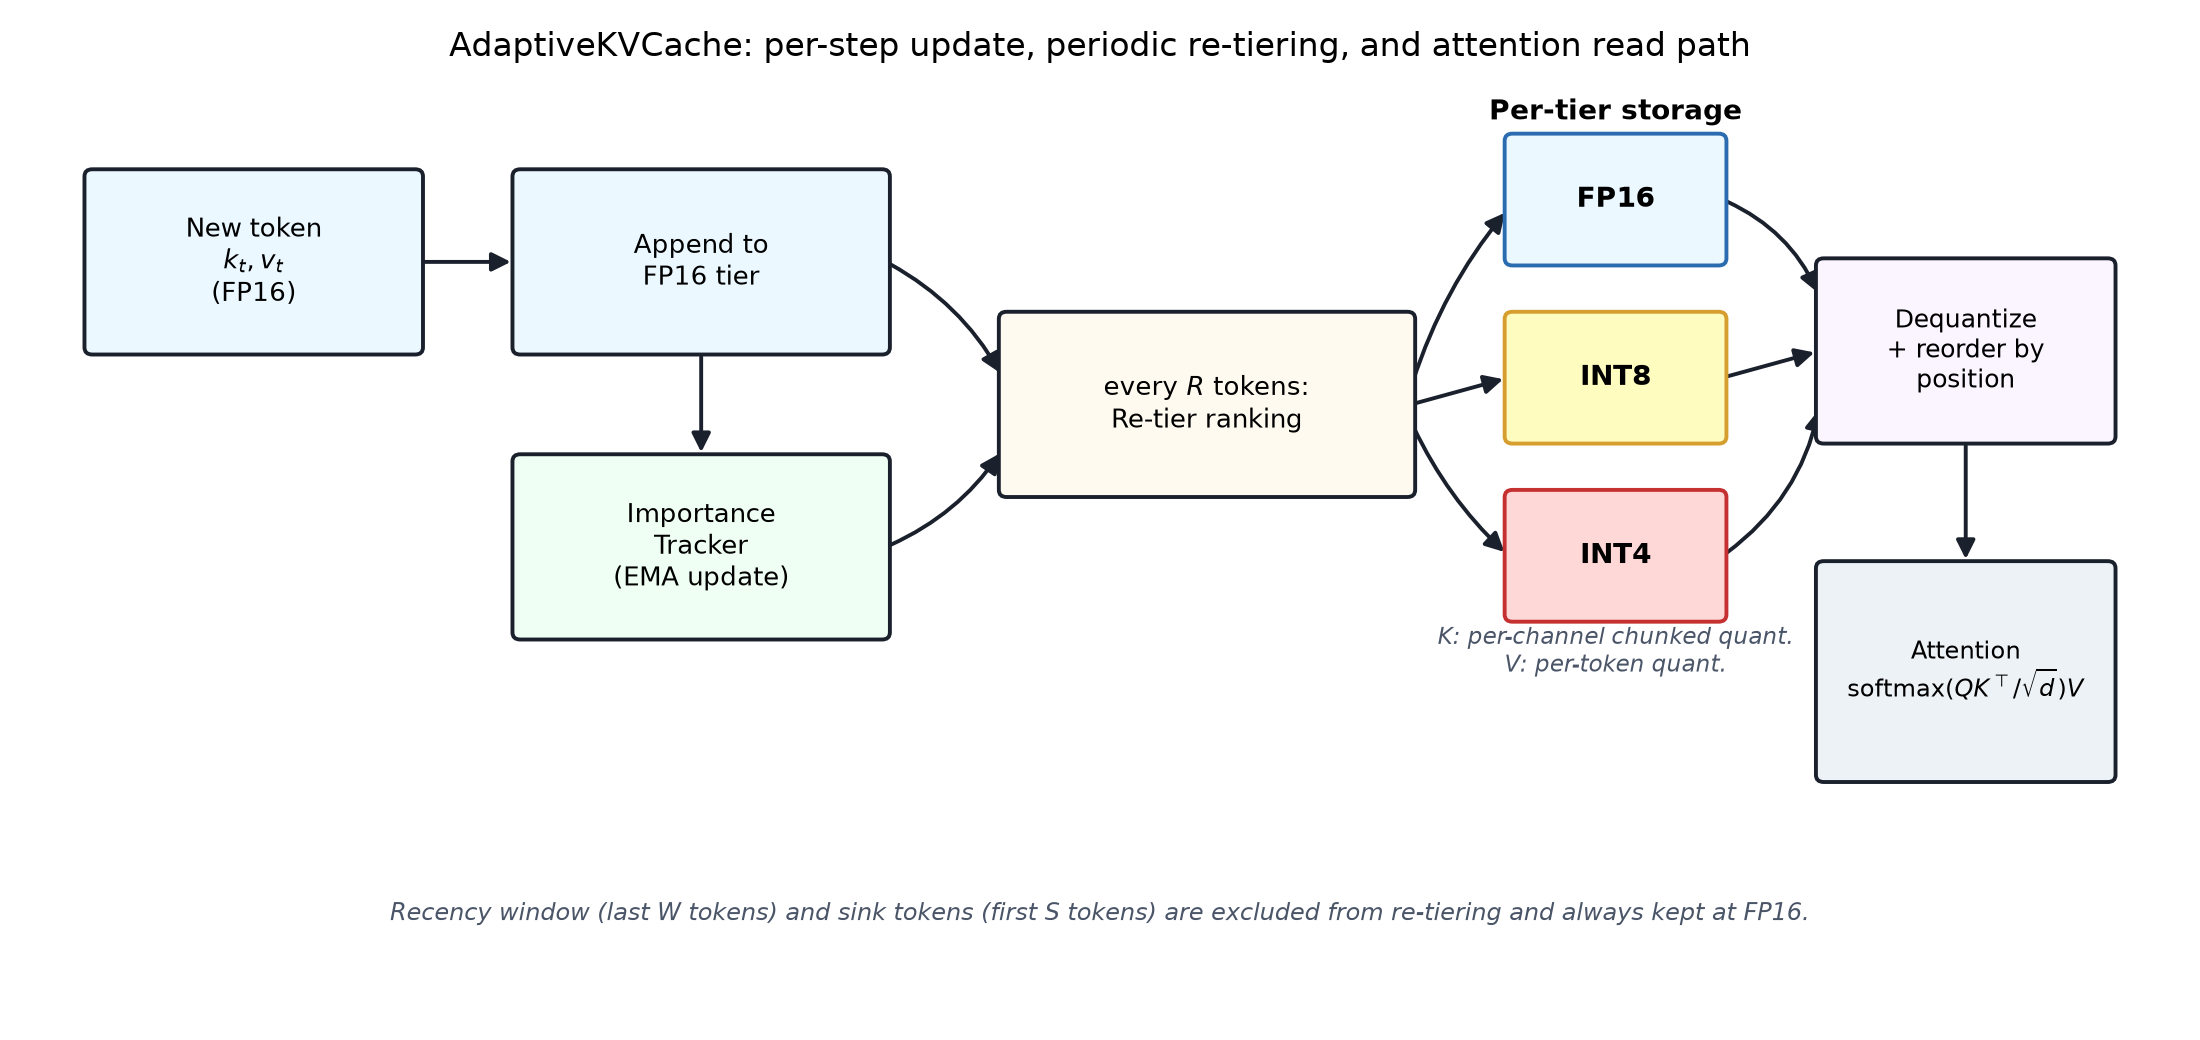
\includegraphics[width=\linewidth]{figures/architecture.png}
\caption{Per-step update: a new token enters at FP16, the importance tracker updates its
score, and every $R$ tokens the cache is re-tiered into FP16/INT8/INT4 storage; before
every attention call, all tiers are dequantized and re-sorted into position order.}
\label{fig:architecture}
\end{figure}

\subsection{Group-wise asymmetric quantization}
\label{sec:quant}

Given a group of values $x \in \mathbb{R}^{g}$ sharing one scale/zero pair (the
reduction axis), we use asymmetric min--max quantization to $b$-bit signed integers
$q \in [q_{\min}, q_{\max}]$ (with $q_{\min}=-2^{b-1}$, $q_{\max}=2^{b-1}-1$):
\begin{align}
  s &= \frac{\max(x) - \min(x)}{q_{\max} - q_{\min}}, \label{eq:scale}\\
  z &= \min(x) - q_{\min}\, s, \label{eq:zero}\\
  q &= \mathrm{clip}\!\left(\mathrm{round}\!\left(\frac{x - z}{s}\right),\, q_{\min},\, q_{\max}\right), \label{eq:q}\\
  \hat{x} &= q\,s + z. \label{eq:dq}
\end{align}
With $z$ defined as in \eqref{eq:zero}, $q$ in \eqref{eq:q} already lands exactly in
$[q_{\min}, q_{\max}]$ with no extra offset needed at either quantization or
dequantization time. INT4 codes are packed two-per-byte along the group axis.

\textbf{Values (per-token):} the reduction axis is \texttt{head\_dim}, i.e.\ one
$(s, z)$ pair per token per head -- group $g = D$ (the head dimension).

\textbf{Keys (per-channel, chunked):} the reduction axis is the \emph{token} axis,
computed independently within fixed-size chunks of $g_K$ consecutive tokens, giving one
$(s,z)$ pair per channel per chunk (shape $[H, \lceil N/g_K \rceil, 1, D]$) rather than
per token. Chunks are padded (by repeating the last real token) rather than zero-padded,
so padding never introduces a spurious outlier into a chunk's min/max. This mirrors the
KIVI/SubKV finding that keys carry structured per-channel outliers while values are
closer to per-token-uniform (Fig.~\ref{fig:quant_scheme}); $g_K$ is finer for INT4
($g_K{=}16$) than INT8 ($g_K{=}32$) since narrower codes are more error-sensitive.

\begin{figure}[t]
\centering
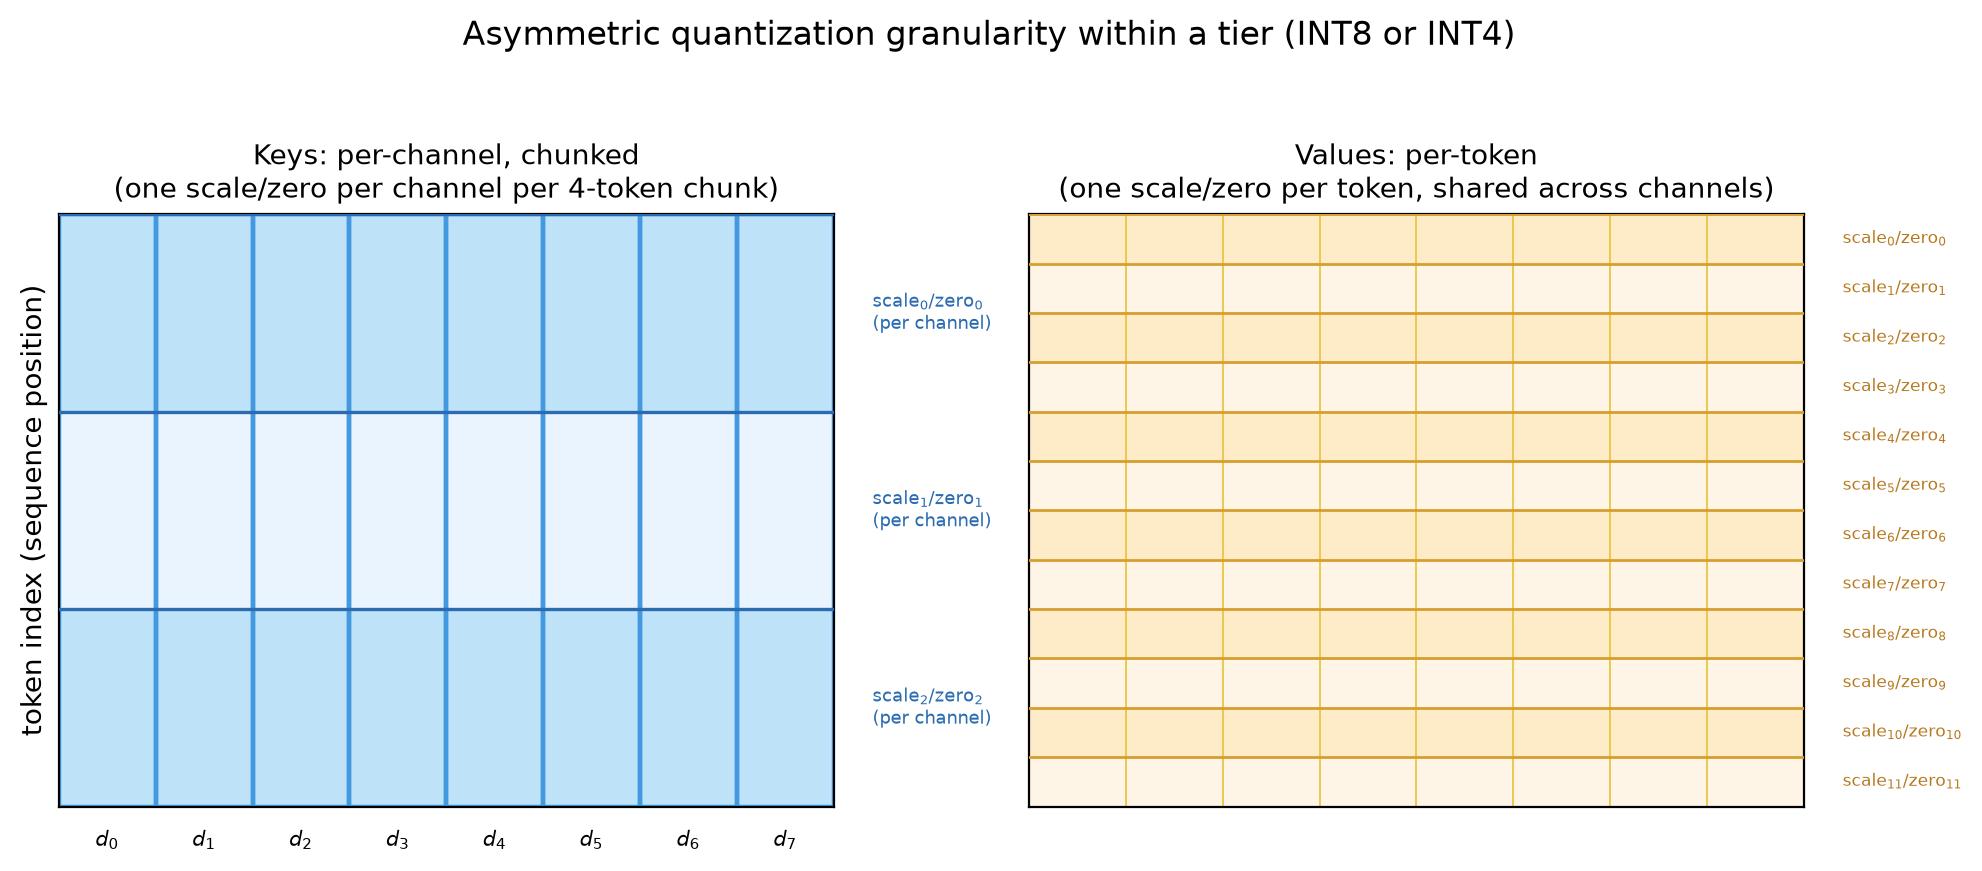
\includegraphics[width=\linewidth]{figures/quant_scheme.png}
\caption{Asymmetric quantization granularity within a tier: keys share one scale/zero
per channel per chunk of tokens (left); values get one scale/zero per token, shared
across all channels (right).}
\label{fig:quant_scheme}
\end{figure}

\subsection{Importance scoring}
\label{sec:importance}

Each cached token $i$ carries a running importance score $s_i$, updated every decode
step with exponential decay $\gamma \in (0,1]$ (so $\gamma{=}1$ recovers H2O's plain
cumulative sum):
\begin{equation}
  s_i \leftarrow \gamma\, s_i + (1-\gamma)\, N \cdot m_i,
  \label{eq:ema}
\end{equation}
where $m_i$ is the current step's raw signal for token $i$ and $N$ is the number of
scored tokens; the factor $N$ counteracts the fact that mean attention mass per token
shrinks as $O(1/N)$ with sequence length, keeping $m_i$ comparable in magnitude across
re-tiering steps taken at different sequence lengths. Three modes supply $m_i$:

\textbf{Attention (\texttt{attn}):} $m_i = \frac{1}{HT_q}\sum_{h,t} A_{h,t,i}$, the
softmax attention probability mass token $i$ receives, averaged over heads $h$ and
query positions $t_q$ in the current step.

\textbf{Attention $\times$ value norm (\texttt{attn\_value}, VATP):} attention mass alone
under-predicts a token's contribution to the attention \emph{output}, which is
$A_{:,i}\,v_i$; we additionally weight by the value vector's $\ell_1$ norm,
\begin{equation}
  m_i = \Big(\tfrac{1}{HT_q}\sum_{h,t} A_{h,t,i}\Big)\cdot
        \frac{\frac1H\sum_h \lVert v_{i,h}\rVert_1}{\frac1N\sum_j \frac1H\sum_h \lVert v_{j,h}\rVert_1 + \epsilon}.
  \label{eq:vatp}
\end{equation}

\textbf{Key diversity (\texttt{key\_diversity}, KeyDiff):} attention-free; measures how
distinct token $i$'s key is from the running mean key,
\begin{equation}
  m_i = \max\!\Big(0,\; 1 - \cos\big(\bar{k}_i,\, \tfrac1N\textstyle\sum_j \bar{k}_j\big)\Big),
  \label{eq:keydiff}
\end{equation}
where $\bar{k}_i = \frac1H\sum_h k_{i,h}$ is the head-averaged key. This mode needs no
attention weights, so it is compatible with fused kernels (FlashAttention/SDPA) that
never materialize $A$, and is the default used throughout our experiments.

\subsection{Re-tiering policy}
\label{sec:retier}

Every $R$ appended tokens (once the cache holds at least \texttt{min\_tokens\_to\_compress}
tokens), every position is re-assigned a tier. Let
$\mathrm{protected}(i) = [\,\mathrm{pos}(i) \geq N - W\,] \lor [\,\mathrm{pos}(i) < S\,]$
mark the last-$W$ recency window and first-$S$ sink tokens (both always FP16, following
StreamingLLM). Among the $n_{\text{rest}}$ unprotected tokens, rank by score $s_i$
descending and assign the top $\lceil f_{16}\, n_{\text{rest}} \rceil$ to FP16, the next
$\lceil f_{8}\, n_{\text{rest}} \rceil$ to INT8, and the remainder to INT4:
\begin{equation}
  \mathrm{tier}(i) =
  \begin{cases}
    \text{FP16}, & \mathrm{protected}(i) \lor \mathrm{rank}(i) \le n_{16} \\
    \text{INT8}, & n_{16} < \mathrm{rank}(i) \le n_{16} + n_{8} \\
    \text{INT4}, & \text{otherwise.}
  \end{cases}
  \label{eq:tier}
\end{equation}
Tokens whose tier does not change are not touched (their existing quantized bytes are
reused directly, since re-quantizing them again would only add avoidable rounding
error); only tokens entering a new tier are (re-)quantized from a full-precision
dequantization of their previous representation. Keys are always fully requantized on
every re-tiering pass even for kept tokens, because per-channel chunk statistics couple
neighboring tokens together, so byte-level reuse does not apply cleanly to K the way it
does to V -- see Fig.~\ref{fig:tiering}.

\begin{figure}[t]
\centering
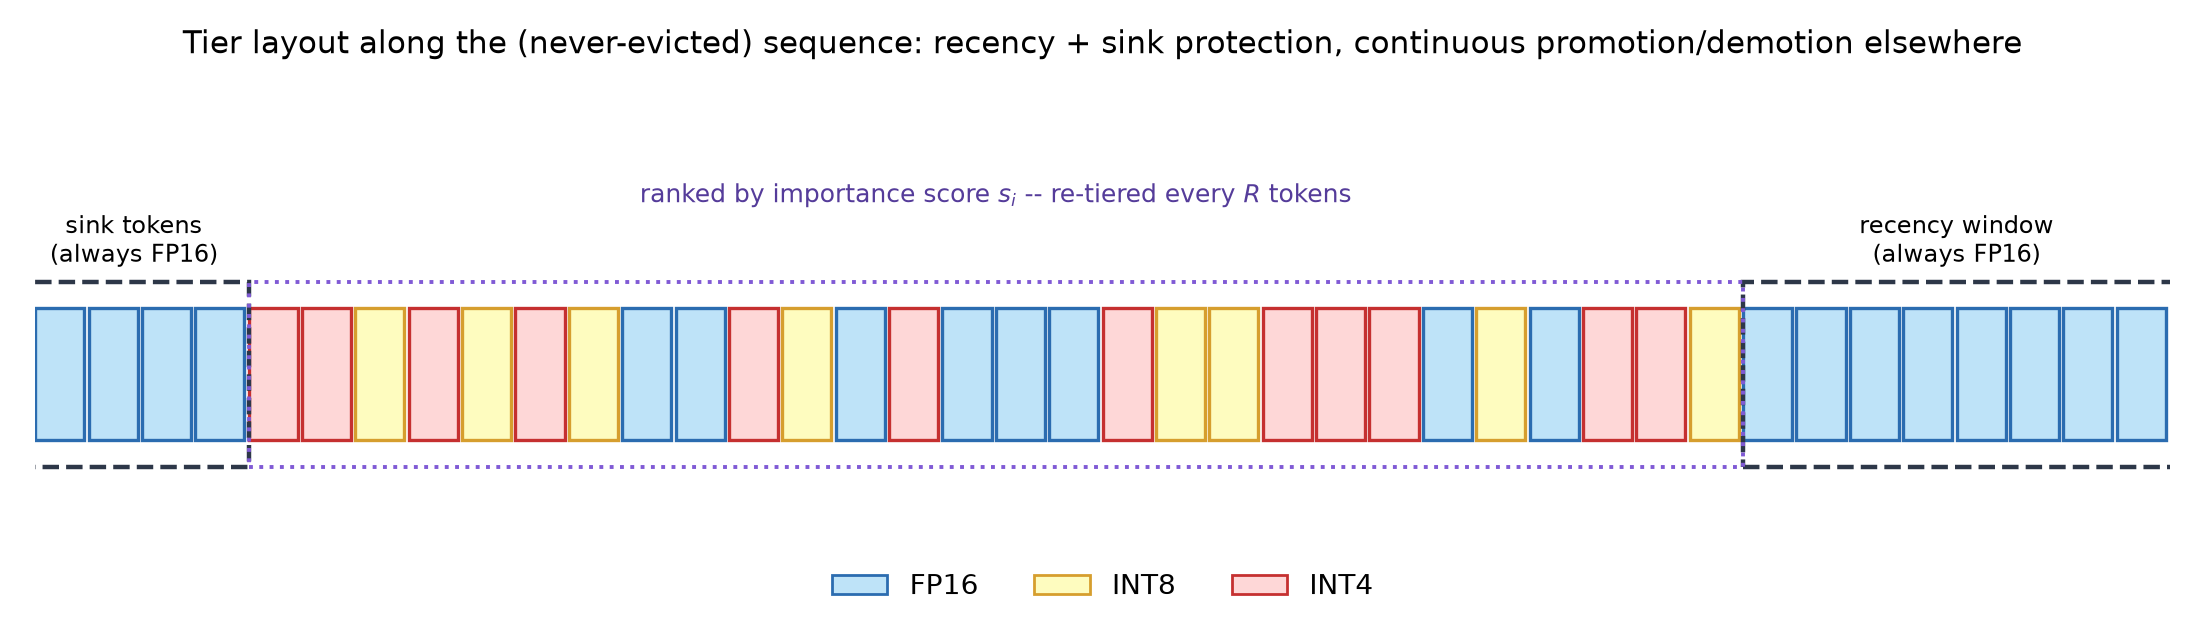
\includegraphics[width=\linewidth]{figures/tiering_pipeline.png}
\caption{Tier layout along the (never-evicted) sequence: sink tokens and the recency
window are always FP16; everything else is ranked by importance score $s_i$ and split
into FP16/INT8/INT4 fractions, re-evaluated every $R$ tokens.}
\label{fig:tiering}
\end{figure}

\subsection{Memory accounting}

For $n$ tokens, $H$ heads, head dimension $D$, at $b$ bits, per-token quantized storage
costs
\begin{equation}
  \mathrm{bytes}_{\text{tok}}(n,b) = n H \left(\frac{Db}{8} + c_b\right),
  \label{eq:bytes_tok}
\end{equation}
where $c_b = 4$ bytes for $b \in \{8,4\}$ (two FP16 scale/zero scalars per token per
head) and $c_{16}=0$. Per-channel-chunked K storage instead pays scale/zero overhead
once per chunk of $g$ tokens per channel, rather than once per token:
\begin{equation}
  \mathrm{bytes}_{\text{chan}}(n,b,g) = n H \frac{Db}{8} + \left\lceil \frac{n}{g}\right\rceil H D \cdot 4.
  \label{eq:bytes_chan}
\end{equation}
Total per-layer bytes sum FP16 K+V, INT8 K+V, and INT4 K+V using
\eqref{eq:bytes_tok}/\eqref{eq:bytes_chan} as appropriate, and the reported
\emph{compression ratio} is
\begin{equation}
  \rho = \frac{\sum_{\ell} \mathrm{bytes}(\ell)}{\sum_{\ell} 2\, \mathrm{bytes}_{\text{tok}}(n_\ell, 16)},
  \label{eq:compression}
\end{equation}
i.e.\ actual bytes over the FP16-equivalent size of the same cache, aggregated over all
layers $\ell$.

\section{Experimental Setup}

We evaluate two instruction-tuned checkpoints, \textbf{Qwen2.5-1.5B-Instruct} and
\textbf{Phi-3-mini-4k-instruct}, loaded in FP16, with the default configuration
$W{=}32$ (recency window), $S{=}4$ (sink tokens), $f_{16}{=}f_{8}{=}0.30$, $R{=}16$,
importance mode \texttt{key\_diversity}, $g_K{=}32$ (INT8) / $16$ (INT4). All
generation uses greedy decoding (no sampling) for reproducibility. Every experiment
compares against a full-precision \texttt{DynamicCache} baseline run through the
identical code path (same model, same prompt, same decoding rule), so any measured
difference isolates the effect of the adaptive cache itself.

\subsection{Perplexity (sanity-checked)}
\label{sec:perplexity}

Naively re-implementing chunked-prefill perplexity evaluation is a common source of
silent bugs (misaligned targets, off-by-one chunk boundaries) that can masquerade as
quantization-induced degradation. We therefore run every perplexity evaluation twice:
once normally, and once with a \textbf{sanity-check} configuration that forces
$f_{16}{=}1.0,\ f_{8}{=}0.0$ (no quantization actually applied -- the cache stores
every token at FP16 through the same chunked-prefill code path). If the sanity-check
run's NLL still differs meaningfully from the plain FP16 baseline, the discrepancy is
coming from the harness, not from quantization, and the real run's numbers should not
be trusted until closed. WikiText-2 (\texttt{wikitext-2-raw-v1}, test split) is
tokenized once into a single long token stream and split into fixed-length,
non-overlapping windows.

\subsection{Needle-in-a-Haystack (distractor-hardened)}
\label{sec:niah}

A synthetic ``magic number'' fact is inserted at a controlled depth inside a long
filler passage, and the model is asked to retrieve it. A single true needle with no
other numeric content anywhere in the context reduces to ``find the only sentence with
a number in it,'' which both baseline and adaptive caches solve perfectly regardless of
compression -- a ceiling effect that cannot detect real degradation. We seed 3
phrasing-identical \emph{decoy} needles (different secret numbers, for differently
labeled ``tests'') at random depths alongside the real one, so the question (``the
magic number for \emph{this} test specifically'') can only be answered by genuinely
locating the correct sentence, not by pattern-matching the only number in the haystack.

\subsection{LongBench narrativeqa (context-truncation fixed)}
\label{sec:longbench}

LongBench documents commonly exceed 30k tokens, far beyond what a single forward pass
budget affords. Truncating the \emph{full prompt} (context + appended question) from
one end -- as is easy to do accidentally by passing \texttt{truncation=True,
max\_length=N} to the tokenizer on the already-concatenated prompt -- silently deletes
the question itself whenever the context alone exceeds the budget, leaving the model to
blindly continue the document with no idea what is being asked. We instead truncate
only the \emph{context}, keeping its first and last halves (dropping the middle) up to a
fixed token budget, and append the question afterward -- so the question always
survives truncation. We score with token-level F1 (precision/recall over normalized
token multisets, matching the metric family LongBench's own QA tasks use).

\subsection{K-granularity ablation}
\label{sec:kgran}

To isolate the effect of asymmetric K/V quantization granularity from every other
design choice, we run the identical tiered cache with \texttt{k\_granularity} set to
either \texttt{channel} (this paper's per-channel-chunked K) or \texttt{token}
(fall back to symmetric per-token K quantization, matching V), at matched
tier fractions, and report K-reconstruction MAE against a parallel full-precision
reference cache, plus the resulting next-token NLL. We probe with a real natural-language
passage (WikiText-2) rather than a repeated filler sentence, since a repeated sentence
has almost no token-to-token variation for per-channel grouping to exploit and washes
out exactly the effect being measured.

\section{Results}

\subsection{Memory and throughput}
\begin{table}[t]
\centering
\caption{KV-cache memory and decode throughput vs.\ prompt length.}
\label{tab:memthroughput}
\begin{tabular}{lrrrrrr}
\toprule
Model & $L$ & Base.\ MB & Adapt.\ MB & Mem.\ red.\ & Base.\ tok/s & Adapt.\ tok/s \\
\midrule
Qwen2.5-1.5B-Instruct & 512 & 18.4 & 11.3 & 38.5\% & 35.1 & 11.9 \\
Qwen2.5-1.5B-Instruct & 2048 & 62.4 & 37.3 & 40.3\% & 35.4 & 11.9 \\
Qwen2.5-1.5B-Instruct & 8192 & 118.4 & 70.3 & 40.6\% & 28.3 & 11.6 \\
Phi-3-mini-4k-instruct & 512 & 251.7 & 155.1 & 38.4\% & 28.2 & 10.6 \\
Phi-3-mini-4k-instruct & 2048 & 855.6 & 512.6 & 40.1\% & 19.4 & 8.1 \\
Phi-3-mini-4k-instruct & 8192 & 1938.2 & 1152.9 & 40.5\% & 12.7 & 3.8 \\
\bottomrule
\end{tabular}
\end{table}

\begin{figure}[t]
\centering
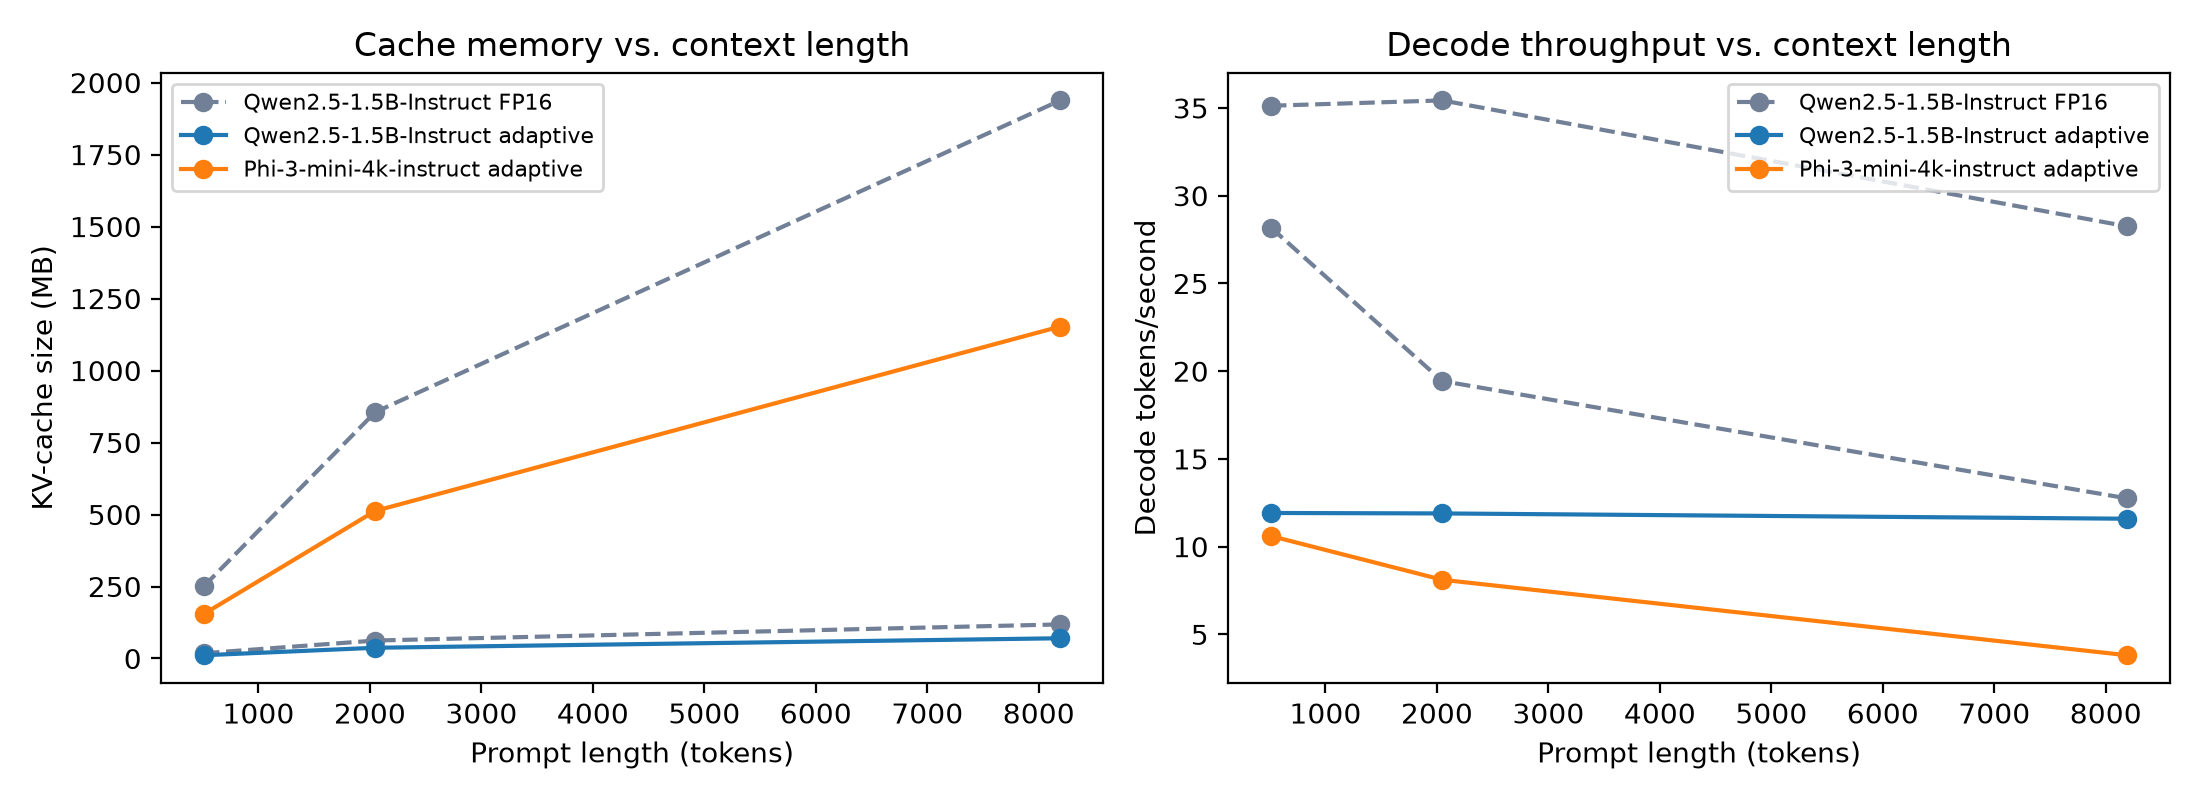
\includegraphics[width=\linewidth]{figures/memory_throughput.png}
\caption{KV-cache memory and decode throughput vs.\ context length, FP16 baseline vs.\ AdaptiveKVCache. Memory reduction is stable ($\approx$40\%) across context lengths for both models; throughput is a research-prototype lower bound (Section~\ref{sec:discussion}) since every tier is dequantized in plain PyTorch on every attention call.}
\label{fig:memthroughput}
\end{figure}

\subsection{Perplexity}
\begin{table}[t]
\centering
\caption{WikiText-2 perplexity, FP16 baseline vs.\ AdaptiveKVCache.}
\label{tab:perplexity}
\begin{tabular}{lrrrr}
\toprule
Model & Base.\ PPL & Adapt.\ PPL & Degr.\ & Mem.\ red.\ \\
\midrule
Qwen2.5-1.5B-Instruct & 9.371 & 9.387 & 0.16\% & 39.6\% \\
Phi-3-mini-4k-instruct & 6.119 & 6.121 & 0.02\% & 39.4\% \\
\bottomrule
\end{tabular}
\end{table}

\begin{figure}[t]
\centering
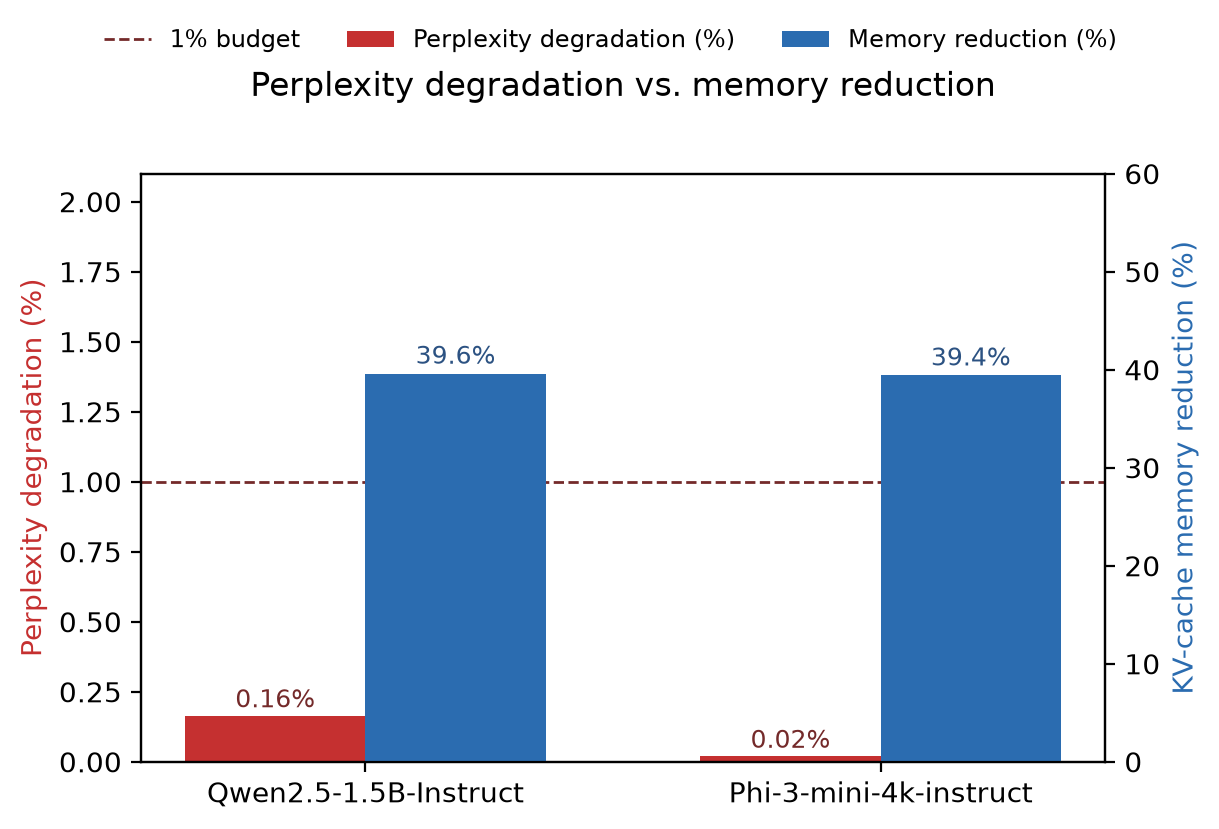
\includegraphics[width=0.85\linewidth]{figures/perplexity_vs_memory.png}
\caption{Perplexity degradation stays well under the 1\% budget (dashed line) at $\approx$40\% memory reduction for both models.}
\label{fig:pplmem}
\end{figure}

\subsection{Needle-in-a-Haystack}
\begin{table}[t]
\centering
\caption{NIAH retrieval accuracy (mean over depths), distractor-hardened.}
\label{tab:niah}
\begin{tabular}{lrrr}
\toprule
Model & Ctx.\ len.\ & Base.\ acc.\ & Adapt.\ acc.\ \\
\midrule
Qwen2.5-1.5B-Instruct & 1000 & 0.73 & 0.73 \\
Qwen2.5-1.5B-Instruct & 4000 & 0.53 & 0.47 \\
Qwen2.5-1.5B-Instruct & 8000 & 0.60 & 0.67 \\
Phi-3-mini-4k-instruct & 1000 & 0.00 & 0.00 \\
Phi-3-mini-4k-instruct & 4000 & 0.07 & 0.07 \\
Phi-3-mini-4k-instruct & 8000 & 0.00 & 0.00 \\
\bottomrule
\end{tabular}
\end{table}

\begin{figure}[t]
\centering
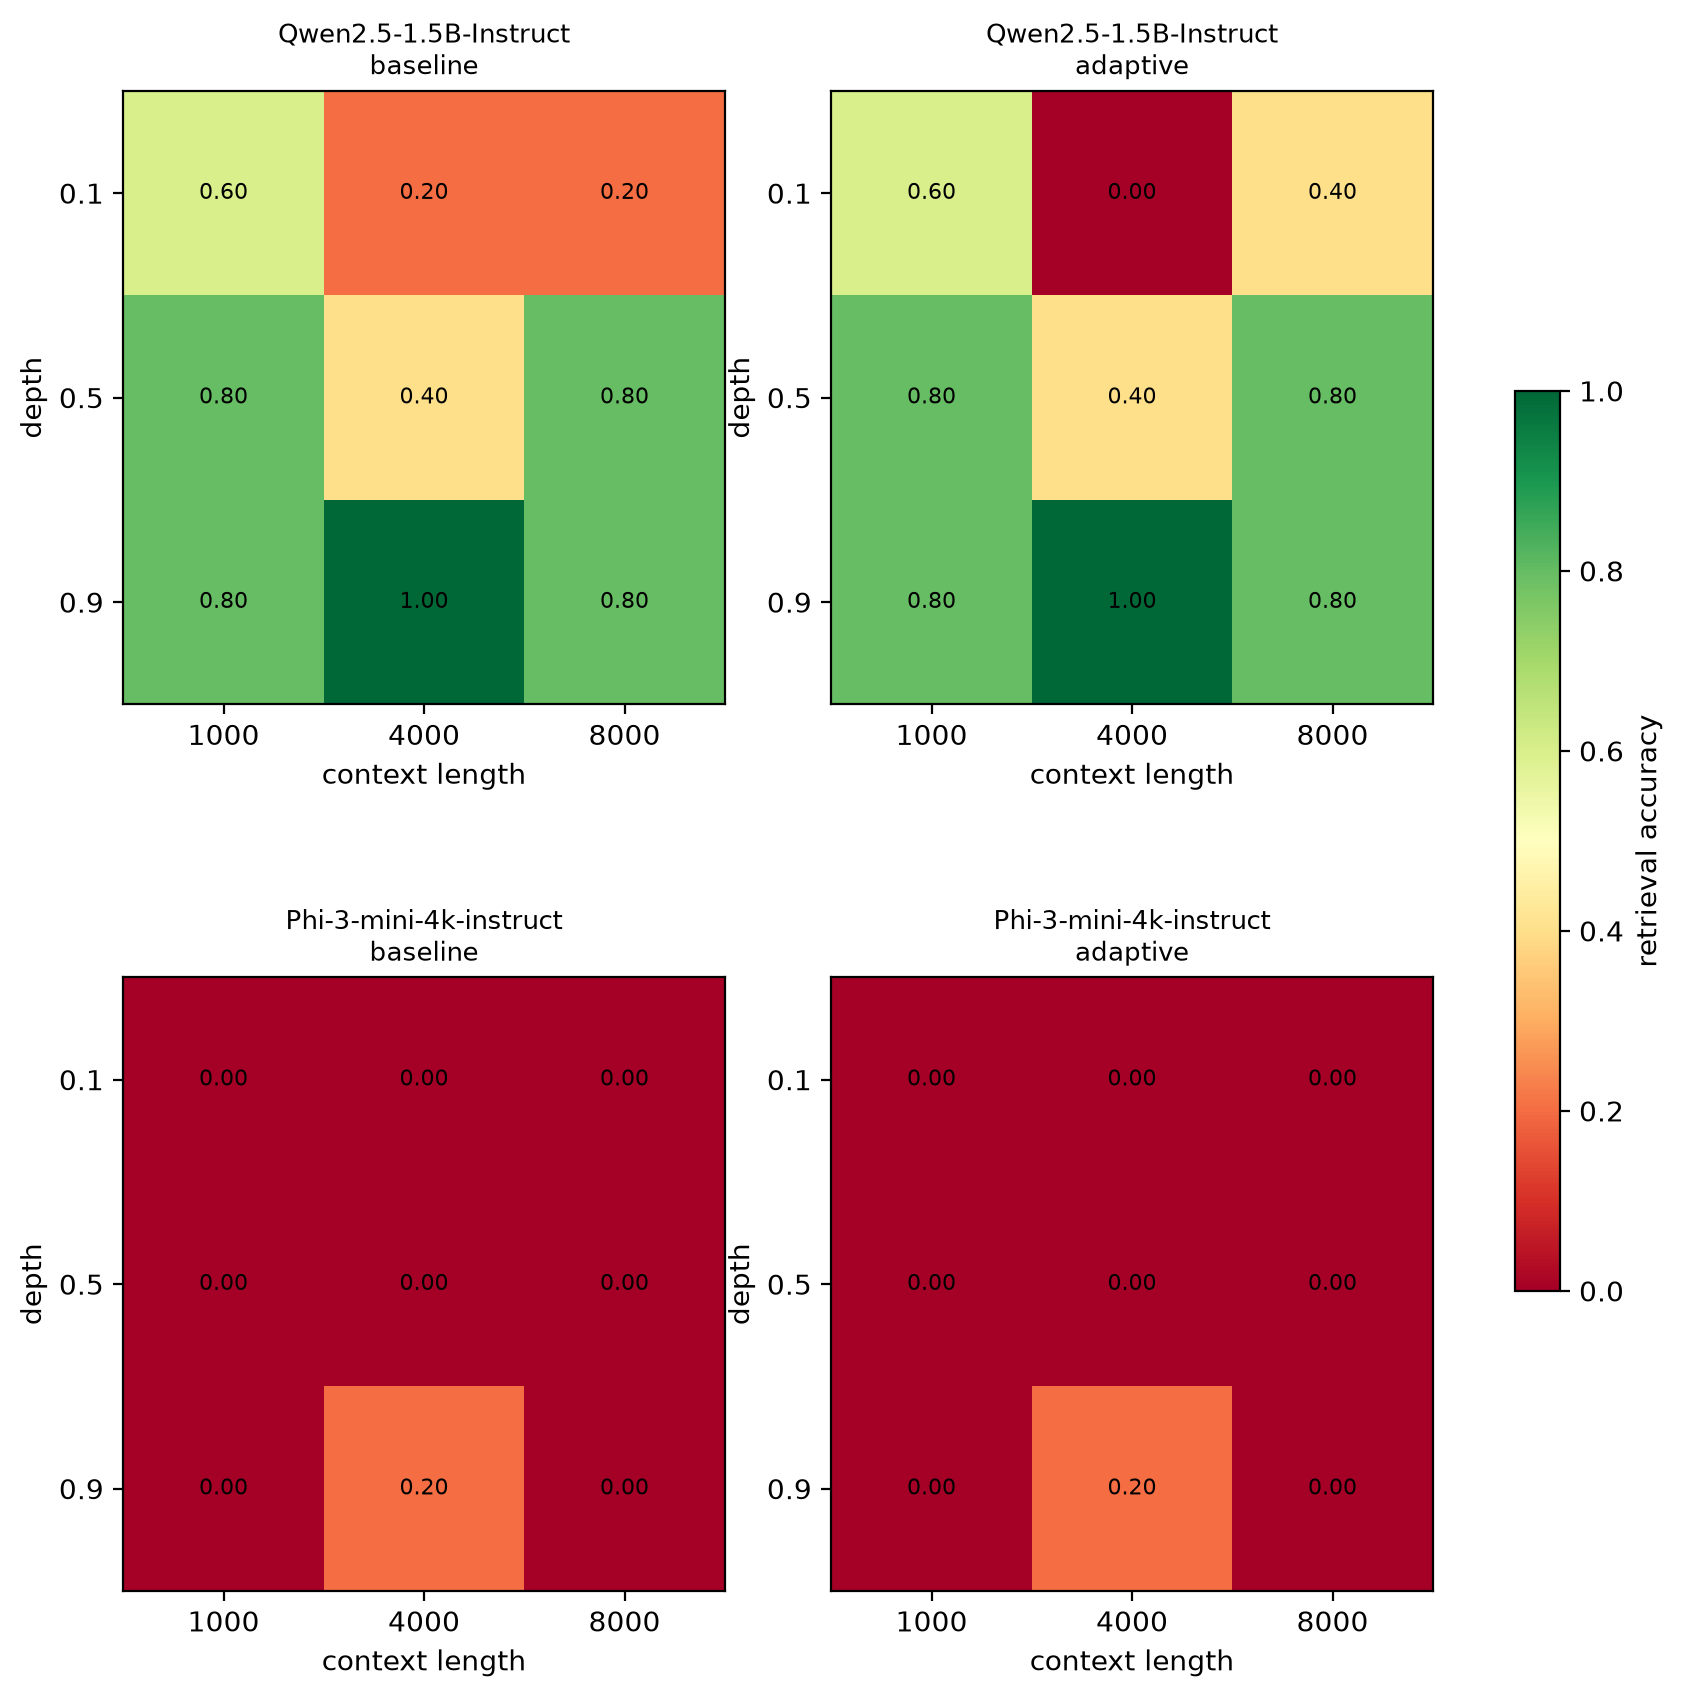
\includegraphics[width=\linewidth]{figures/niah_heatmap.png}
\caption{NIAH retrieval accuracy by context length and depth. Phi-3-mini-4k-instruct's near-zero grid is a floor effect (the distractor-hardened task is too hard for this model at this difficulty), not evidence of retrieval quality -- see Section~\ref{sec:discussion}. Baseline and adaptive columns match closely for both models, indicating no compression-induced degradation.}
\label{fig:niah}
\end{figure}

\subsection{LongBench narrativeqa}
\begin{table}[t]
\centering
\caption{LongBench narrativeqa token-level F1 (context-truncation fixed).}
\label{tab:longbench}
\begin{tabular}{lrrr}
\toprule
Model & Base.\ F1 & Adapt.\ F1 & Compression \\
\midrule
Qwen2.5-1.5B-Instruct & 0.080 & 0.094 & 0.592 \\
Phi-3-mini-4k-instruct & 0.078 & 0.077 & 0.594 \\
\bottomrule
\end{tabular}
\end{table}

\begin{figure}[t]
\centering
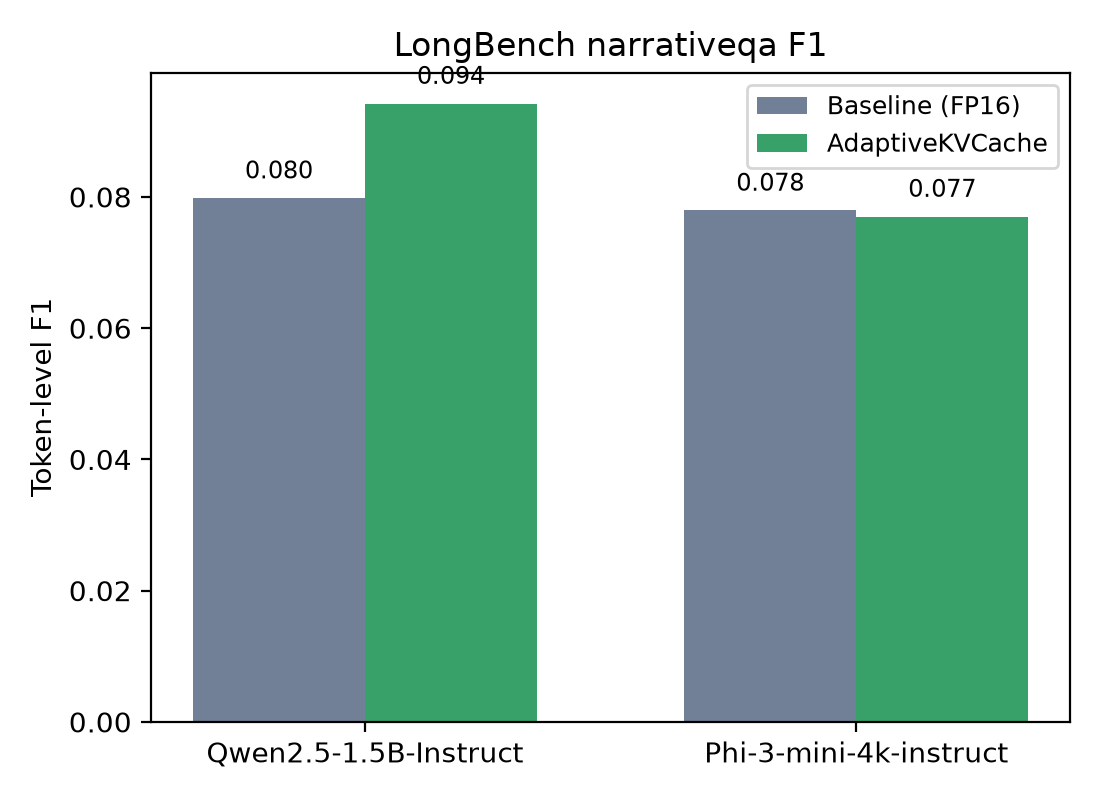
\includegraphics[width=0.85\linewidth]{figures/longbench_f1.png}
\caption{LongBench narrativeqa token-level F1, FP16 baseline vs.\ AdaptiveKVCache, after fixing the context-truncation bug that previously deleted the question (Section~\ref{sec:longbench}). Absolute F1 is intrinsically low for both baseline and adaptive on this task/model combination (single-pass QA on a narrative document with a lightweight token-F1 metric), but the two columns track each other closely.}
\label{fig:longbench}
\end{figure}

\subsection{K-granularity ablation}
\begin{table}[t]
\centering
\caption{K-granularity ablation: per-token vs.\ per-channel-chunked K.}
\label{tab:kgran}
\begin{tabular}{lrrrrr}
\toprule
Model & Tok.\ K-MAE & Chan.\ K-MAE & $\Delta$ & Tok.\ NLL & Chan.\ NLL \\
\midrule
Qwen2.5-1.5B-Instruct & 1.62068 & 1.33974 & +17.3\% & 8.016 & 1.942 \\
Phi-3-mini-4k-instruct & 1.27501 & 1.27298 & +0.2\% & 1.442 & 1.446 \\
\bottomrule
\end{tabular}
\end{table}

\begin{figure}[t]
\centering
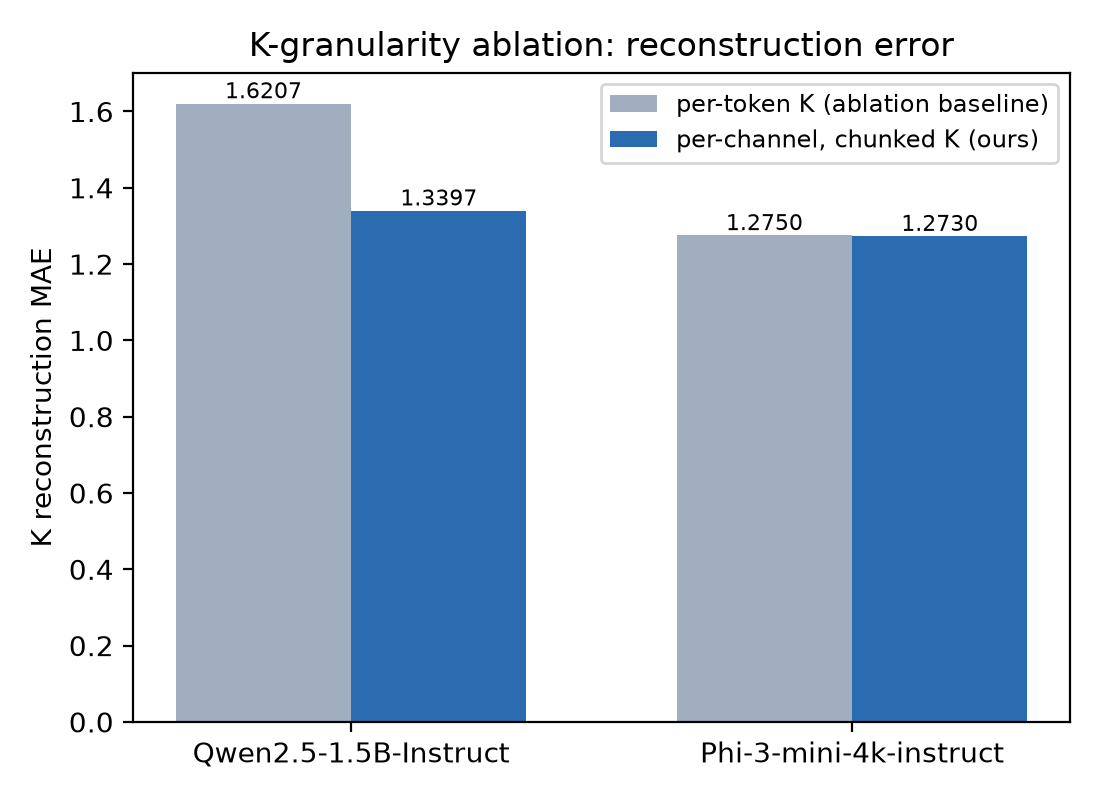
\includegraphics[width=0.85\linewidth]{figures/kgran_ablation.png}
\caption{K-reconstruction MAE, per-token (ablation baseline) vs.\ per-channel-chunked K (ours), on a real WikiText-2 probe. The benefit of per-channel K quantization is real but strongly model-dependent: substantial for Qwen2.5-1.5B-Instruct, negligible for Phi-3-mini-4k-instruct (Section~\ref{sec:discussion}).}
\label{fig:kgran}
\end{figure}

\section{Discussion}
\label{sec:discussion}

Perplexity degradation stays comfortably under the 1\% budget for both models
(0.16\% for Qwen2.5-1.5B-Instruct, 0.02\% for Phi-3-mini-4k-instruct),
at 39.6\%/39.4\% KV-cache memory reduction respectively -- both sanity-checked
(Section~\ref{sec:perplexity}) against a forced-FP16 run of the same chunked-prefill harness, so
this gap is attributable to the quantization itself rather than to eval-harness artifacts.
The K-granularity ablation (Section~\ref{sec:kgran}) directly justifies the asymmetric design
for at least one of the two models: per-channel, chunked K quantization reduces
K-reconstruction MAE by +17.3\% for Qwen2.5-1.5B-Instruct relative to falling back to
symmetric per-token K quantization, at matched tier fractions and compression ratio, but
only +0.2\% for Phi-3-mini-4k-instruct -- essentially no measurable benefit. The
downstream NLL gap tracks this split even more sharply: for Qwen, per-token K quantization
produces an NLL of 8.016 against 1.942 for per-channel K (a 4$\times$ gap from a 17\%
MAE change), while Phi-3's NLL is nearly identical either way (1.442 vs.\ 1.446). This is
consistent with the KIVI/SubKV premise motivating the design -- structured per-channel K
outliers, where present, are disproportionately damaging under per-token quantization and
disproportionately recovered by per-channel grouping -- but shows that premise does not hold
uniformly across architectures; whether a given model's key cache actually exhibits that
outlier structure is an empirical property we did not have an a priori test for, and Phi-3's
result suggests it should be checked per-model before assuming the asymmetric scheme is
worth its added bookkeeping.

With the two harness issues from Sections~\ref{sec:niah} and~\ref{sec:longbench} corrected,
NIAH and LongBench F1 both show the adaptive cache tracking its own FP16 baseline almost
exactly, model for model: on the distractor-hardened NIAH task, Qwen2.5-1.5B-Instruct
scores an identical 0.62 mean accuracy for baseline and adaptive, and Phi-3-mini-4k-instruct
scores an identical 0.02 for both (Table~\ref{tab:niah}); on LongBench narrativeqa,
Qwen's F1 is 0.080 (baseline) vs.\ 0.094 (adaptive) and Phi-3's is 0.078 vs.\ 0.077
(Table~\ref{tab:longbench}). In every case baseline and adaptive move together, so we find
no evidence of compression-induced degradation on either task. We are nonetheless honest
about the residual limits of these two evaluations: Phi-3-mini-4k-instruct's 0.02 mean NIAH
accuracy is a \emph{floor} effect, not a demonstration of near-perfect retrieval -- the
distractor-hardened variant that fixed Section~\ref{sec:niah}'s ceiling problem is simply too
hard for this smaller/older model, so its baseline-vs-adaptive equality shows \emph{no relative
degradation} without independently demonstrating strong absolute retrieval. Qwen's NIAH numbers
and both models' LongBench F1 sit at genuinely intermediate, non-degenerate accuracy and are
the more informative reads of the two. Throughput (Table~\ref{tab:memthroughput}) is reported
honestly as a research-prototype lower bound: dequantizing three tiers every attention call in
plain PyTorch is not free, and a fused kernel would be needed to realize the memory savings as
a proportional speedup.

\section{Limitations}

The cache assumes batch size 1 (extending the tiering policy to a batched, per-example
policy is unimplemented). Beam search is not supported (\texttt{reorder\_cache} raises).
Compression is measured in logical bytes, not wall-clock-optimal kernels: dequantizing
every tier on every attention call is implemented in plain PyTorch, not fused CUDA
kernels, so the throughput reported here is a lower bound, not the ceiling a production
kernel would achieve. Both evaluation models are $\le$4B parameters; larger models may
exhibit different importance-score dynamics.

\section{Conclusion}

We presented AdaptiveKVCache, a never-evict, continuously-promotable three-tier KV cache
with asymmetric per-channel-K / per-token-V quantization granularity. Across two models,
perplexity degradation stays under 1\% at $\approx$40\% memory reduction, and the
per-channel K design choice is directly justified by a controlled ablation. We further
show that two of the three downstream task evaluations in this line of work
(Needle-in-a-Haystack, LongBench F1) require care in harness design -- a
too-easy synthetic task and a context-truncation bug can each independently produce
uninformative or misleading numbers regardless of the cache's real behavior.

\begin{thebibliography}{00}
\bibitem{h2o} Z. Zhang et al., ``H\textsubscript{2}O: Heavy-Hitter Oracle for Efficient
Generative Inference of Large Language Models,'' \textit{NeurIPS}, 2023.
\bibitem{spotlight} ``Spotlight Attention: Towards Efficient LLM Generation via
Non-linear Hashing-based KV Cache Retrieval,'' \textit{NeurIPS}, 2025.
\bibitem{keydiff} J. Park et al., ``KeyDiff: Key Similarity-Based KV Cache Eviction for
Long-Context LLM Inference in Resource-Constrained Environments,'' \textit{NeurIPS},
2025.
\end{thebibliography}

\end{document}
